\documentclass[utf8,compress]{beamer}
\usepackage{irbookslide}
\usepackage{irilmenau2}
\usepackage{url}
\usepackage{fontspec} % zahteva paket euenc
\usepackage{xunicode}
\usepackage{xltxtra}
\usepackage{polyglossia}
\usepackage[cache=false]{minted}
\usepackage{xcolor,colortbl}
\usepackage{textcomp}
\usepackage{unicode-math}

\title{Dizajn algoritama i rekurzija}
\subtitle{\tiny{Slajdovi za predmet Osnove programiranja}}
\subject{Osnove programiranja}
\institute{Katedra za informatiku, Fakultet tehničkih nauka, Novi Sad}
\date{2018.}

\begin{document}

% da pygmentize ne uokviruje crvenom bojom nepoznate karaktere
\expandafter\def\csname PY@tok@err\endcsname{}

\frame{\titlepage}

\frame{
  \frametitle{Ciljevi}
  \begin{itemize}
    \item osnovne tehnike za analizu efikasnosti algoritama
    \item pojam pretraživanja, linearna i binarna pretraga
    \item rekurzivne funkcije
    \item pojam sortiranja; selection sort i merge sort
    \item analiza algoritama; reizračunljivi i nerešivi problemi
  \end{itemize}
}

\section[Pretraga]{Pojam pretraživanja}

\frame{
  \frametitle{Pretraživanje}
  \begin{itemize}
    \item \myblue{pretraživanje} je proces pronalaženja date vrednosti u kolekciji podataka
    \item primer: program za evidentiranje studenata
    \begin{itemize}
      \item pronalaženje podataka o studentu na osnovu broja indeksa
    \end{itemize}
  \end{itemize}
}

\begin{frame}[fragile]
  \frametitle{Primer pretrage}
  \begin{itemize}
    \item funkcija za pretragu
  \end{itemize}
\begin{minted}{python}
def search(x, nums):
    # nums je lista brojeva, x je broj koji se traži
    # vraća indeks u listi gde se nalazi x,
    # ako x nije u listi vraća -1
\end{minted}
  \begin{itemize}
    \item primeri upotrebe:
  \end{itemize}
\begin{minted}{python}
>>> search(4, [3, 1, 4, 2, 5])
2
>>> search(7, [3, 1, 4, 2, 5])
-1
\end{minted}
\end{frame}

\begin{frame}[fragile]
  \frametitle{Pretraga i Python}
  \begin{itemize}
    \item testiranje da li se \texttt{x} nalazi u sekvenci: operator \texttt{in}
  \end{itemize}
\begin{minted}{python}
if x in nums:
    # uradi nešto
\end{minted}
  \begin{itemize}
    \item pozicija \texttt{x} u listi pomoću funkcije \texttt{index}
  \end{itemize}
\begin{minted}{python}
>>> nums = [3, 1, 4, 2, 5]
>>> nums.index(4)
2
\end{minted}
\end{frame}

\begin{frame}[fragile]
  \frametitle{Naša funkcija vs Python funkcija}
  \begin{itemize}
    \item naša funkcija vraća -1 ako ne nađe element u listi
    \item Python-ova funkcija \texttt{index} baca izuzetak ako ne nađe element u listi
    \item mogli bismo napraviti naš \texttt{search} tako da koristi \texttt{index},
    \item hvata izuzetak i vraća -1 u tom slučaju
  \end{itemize}
\begin{minted}{pyton}
def search(x, nums):
    try:
        return nums.index(x)
    except:
        return -1
\end{minted}
\end{frame}

\begin{frame}[fragile]
  \frametitle{Naša funkcija vs Python funkcija $_2$}
  \begin{itemize}
    \item prethodni primer može da posluži,
    \item ali nas zanima kako Python implementira \texttt{index}
  \end{itemize}
\end{frame}

\section[Linearna]{Linearna pretraga}

\begin{frame}[fragile]
  \frametitle{Strategija 1: linearna pretraga}
  \begin{itemize}
    \item primer: data nam je neuređena lista brojeva
    \item zanima nas da li je broj 13 u toj listi
    \item kako da to ispitamo? \\ \ \\
    \item krenemo od početka liste
    \item poredimo svaki element liste sa 13
    \item ako naiđemo na 13, vratimo indeks
    \item ako dođemo do kraja liste i ne nađemo 13, vratimo -1
  \end{itemize}
\end{frame}

\begin{frame}[fragile]
  \frametitle{Linearna pretraga}
  \begin{itemize}
    \item \myblue{linearna pretraga}: prolazimo redom kroz sve elemente liste
    \item prekidamo pretragu kad nađemo podatak ili kada dođemo do kraja liste
  \end{itemize}
\begin{minted}{python}
def search(x, nums):
    for i in range(len(nums)):
        if nums[i] == x: # pronađen
            return i
    return -1  # došli do kraja, nije pronađen
\end{minted}
  \begin{itemize}
    \item jednostavan algoritam
    \item pristojne performanse za male (kratke) liste
  \end{itemize}
\end{frame}

\begin{frame}[fragile]
  \frametitle{Linearna pretraga $_2$}
  \begin{itemize}
    \item Pythonov operator \texttt{in} i funkcija \texttt{index} vrše linearnu pretragu
    \item ako je lista vrlo velika, pretraga može da traje \\ \ \\
    \item isplati se organizovati podatke tako da ne testiramo sve elemente liste
  \end{itemize}
\end{frame}

\section[Binarna]{Binarna pretraga}

\begin{frame}[fragile]
  \frametitle{Binarna pretraga}
  \begin{itemize}
    \item ako su podaci sortirani, ne moramo testirati sve elemente liste
    \item kad naiđemo na element koji je veći od tražene vrednosti
    \item ne moramo testirati elemente iza njega! \\ \ \\
    \item u proseku, možemo uštedeti polovinu testova
  \end{itemize}
\end{frame}

\begin{frame}[fragile]
  \frametitle{Binarna pretraga $_2$}
  \begin{itemize}
    \item igra pogađanja zamišljenog broja:
    \item igrač A zamisli broj između 1 i 100, a igrač B ga pogađa
    \item za svaki pokušaj igrač A kaže da li je zamišljeni broj veći 
      ili manji od broja koji je pokušao igrač B \\ \ \\
    \item isplati se prvo probati 50; tri ishoda:
    \item[a)] pogodili smo broj :)
    \item[b)] ako je odgovor da je broj veći od 50, odbacujemo opseg 1-50
    \item[c)] u suprotnom odbacujemo opseg 50-100
    \item ako je odgovor pod b), sledeći pokušaj nam je broj 75...
  \end{itemize}
\end{frame}

\begin{frame}[fragile]
  \frametitle{Binarna pretraga $_2$}
  \begin{itemize}
    \item svaki put kao pogodak biramo sredinu trenutnog opsega
    \item time polovimo opseg
    \item ovakav pristup se zove \myblue{binarna pretraga} \\ \ \\
    \item binarna jer delimo opseg na dva dela
  \end{itemize}
\end{frame}

\begin{frame}[fragile]
  \frametitle{Binarna pretraga $_3$}
  \begin{itemize}
    \item ovo možemo koristiti za naš problem
    \item treba da pamtimo indekse za početak i kraj tekućeg opsega
    \item inicijalne vrednosti indeksa:
    \begin{itemize}
      \item \texttt{low = 0}
      \item \texttt{high = len(list)-1}
    \end{itemize}
  \end{itemize}
\end{frame}

\begin{frame}[fragile]
  \frametitle{Binarna pretraga $_4$}
  \begin{itemize}
    \item glavni deo algoritma je petlja koja poredi srednji element opsega sa \texttt{x}
    \item ako je \texttt{x} manji od srednjeg, \\ \texttt{high} se pomera na kraj prve polovine
    \item ako je \texttt{x} veći od srednjeg, \\ \texttt{low} se pomera na početak druge polovine
    \item ako je \texttt{x} jednak srednjem -- našli smo broj \\ \ \\
    \item petlja se završava ako
    \begin{itemize}
      \item smo našli \texttt{x}
      \item nema više elemenata za test (\texttt{low > high})
    \end{itemize}
  \end{itemize}
\end{frame}

\begin{frame}[fragile]
  \frametitle{Binarna pretraga $_5$}
\begin{minted}{python}
def search(x, nums):
    low = 0
    high = len(nums) - 1
    while low <= high:        # dok opseg nije širok 0
        mid = (low + high)//2 # indeks srednjeg elementa
        item = nums[mid]
        if x == item:         # ako smo ga našli
            return mid
        elif x < item:        # x je u prvoj polovini
            high = mid - 1
        else:                 # x je u gornjoj polovini
            low = mid + 1
    return -1                 # nismo našli x
\end{minted}
\end{frame}

\section[Poređenje]{Poređenje algoritama}

\begin{frame}[fragile]
  \frametitle{Poređenje algoritama}
  \begin{itemize}
    \item koji algoritam je bolji -- linearna ili binarna pretraga?
    \begin{itemize}
      \item linearna je jednostavnija
      \item binarna je efikasnija jer ne testira sve elemente
    \end{itemize}
    \item (intuitivno) možemo očekivati da linearna pretraga radi 
      bolje za kratke liste, a binarna za dugačke
    \item kako da budemo sigurni?
  \end{itemize}
\end{frame}

\begin{frame}[fragile]
  \frametitle{Poređenje algoritama $_2$}
  \begin{itemize}
    \item jedan način: da probamo oba algoritma za liste različite dužine 
       i merimo vreme
    \begin{itemize}
      \item linearna je brža za liste kraće od 10 elemenata
      \item mala razlika za liste od 10-1000 elemenata
      \item binarna je znatno brža za liste od 1000+ elemenata \\
        (za milion elemenata: binarna u proseku 0.0003s, linearna 2.5s)
    \end{itemize}
  \end{itemize}
\end{frame}

\begin{frame}[fragile]
  \frametitle{Poređenje algoritama $_3$}
  \begin{itemize}
    \item ovakvi testovi zavise od
    \begin{itemize}
      \item vrste računara
      \item količine memorije
      \item brzine procesora
      \item itd.
    \end{itemize}
    \item umesto štoperice, možemo da analiziramo algoritme
    \item algoritam koji obavi manji broj \myblue{koraka} je brži
  \end{itemize}
\end{frame}

\begin{frame}[fragile]
  \frametitle{Poređenje algoritama $_4$}
  \begin{itemize}
    \item kako brojimo ,,korake`` u algoritmu?
    \item posmatramo zavisnost broja koraka od veličine kolekcije 
      podataka ili složenosti proračuna \\ \ \\
    \item za pretragu: složenost zavisi od veličine kolekcije
  \end{itemize}
\end{frame}

\begin{frame}[fragile]
  \frametitle{Poređenje algoritama $_5$}
  \begin{itemize}
    \item koliko koraka je potrebno za pretragu u listi dužine $n$? \\ \ \\
    \item šta se dešava kada $n$ postane veliko?
  \end{itemize}
\end{frame}

\begin{frame}[fragile]
  \frametitle{Poređenje algoritama $_6$}
  \begin{itemize}
    \item za linearnu pretragu:
    \begin{itemize}
      \item za listu od 10 elemenata -- max 10 poređenja
      \item za listu od 20 elemenata -- max 20 poređenja
      \item za listu od 30 elemenata -- max 30 poređenja \\ \ \\
    \end{itemize}
    \item broj operacija \myblue{linearno zavisi} od dužine liste $n$
    \item $\rightarrow$ algoritam koji ima linearnu vremensku zavisnost
  \end{itemize}
\end{frame}

\begin{frame}[fragile]
  \frametitle{Poređenje algoritama $_7$}
  \begin{itemize}
    \item za binarnu pretragu:
    \begin{itemize}
      \item neka lista ima 16 elemenata; u svakom ciklusu polovina se 
        eliminiše -- prvi put eliminiše se 8 elemenata
      \item nakon drugog ciklusa ostane još 4 elementa
      \item nakon trećeg ciklusa ostane još 2 elementa
      \item nakon četvrtog ciklusa ostane 1 element \\ \ \\
    \end{itemize}
    \item ako binarna pretraga obavi $i$ ciklusa
    \item može da pronađe element u listi dužine $2^i$
  \end{itemize}
\end{frame}

\begin{frame}[fragile]
  \frametitle{Poređenje algoritama $_8$}
  \begin{itemize}
    \item koliko elemenata se testira za listu dužine $n$?
    \item treba rešiti $n = 2^i$ po $i$, odnosno
    \item $i = log_2 n$ \\ \ \\
    \item binarna pretaga ima \myblue{logaritamsku} vremensku zavisnost
    \item vreme potrebno za pronalaženje raste sa logaritmom dužine liste
  \end{itemize}
\end{frame}

\begin{frame}[fragile]
  \frametitle{Poređenje algoritama $_8$}
  \begin{itemize}
    \item telefonski imenik Njujorka: 12 miliona imena
    \item pronalaženje datog imena u imeniku: 
    \item najviše $log_2 12000000 = 24$ pokušaja! \\ \ \\
    \item za linearnu pretragu treba u proseku 6000000 pokušaja
  \end{itemize}
\end{frame}

\begin{frame}[fragile]
  \frametitle{Linearna vs logaritamska vs eksponencijalna funkcija}
  \begin{center}
    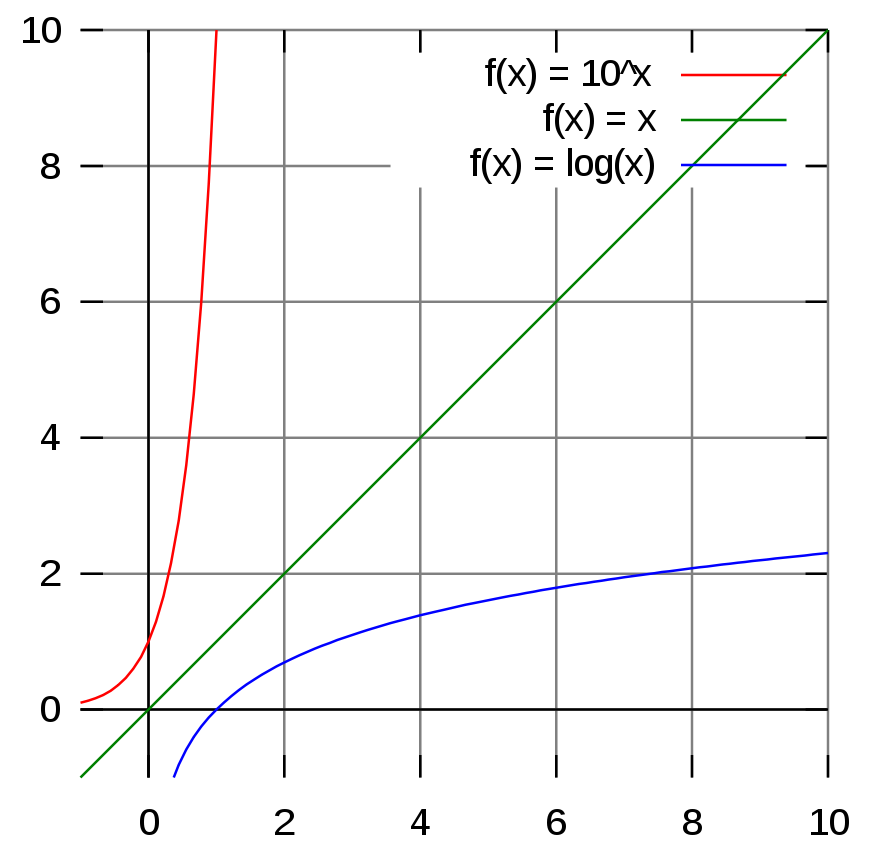
\includegraphics[width=7cm]{pic25}
  \end{center}
\end{frame}

\begin{frame}[fragile]
  \frametitle{Pretraga u Pythonu}
  \begin{itemize}
    \item zašto Python koristi linearnu pretragu?
    \item binarna pretraga očekuje sortiranu listu
    \item ako lista nije sortirana, prvo se mora sortirati
  \end{itemize}
\end{frame}

\section[Rekurzija]{Rekurzija}

\begin{frame}[fragile]
  \frametitle{Podeli i vladaj}
  \begin{itemize}
    \item binarna pretraga deli problem na dva dela
    \item princip \myblue{podeli i vladaj} (divide et impera):
    \item podeli problem na potprobleme koji su manja verzija početnog
  \end{itemize}
\end{frame}

\begin{frame}[fragile]
  \frametitle{Podeli i vladaj: binarna pretraga}
  \begin{itemize}
    \item za binarnu pretragu početni opseg je cela lista
    \item testiramo srednji element...
    \item ako smo pogodili -- kraj
    \item ako nismo -- biramo polovinu i \myblue{ponavljamo} pretragu
  \end{itemize}
\end{frame}

\begin{frame}[fragile]
  \frametitle{Podeli i vladaj: binarna pretraga $_2$}
\begin{minted}{python}
def search(x, nums, low, high):
    if low > high:
        return -1
    mid = (low + high)//2
    if x == nums[mid]:
        return mid
    elsif x < nums[mid]:
        search(x, nums, low, mid-1)
    else:
        search(x, nums, mid+1, high)
\end{minted}
  \begin{itemize}
    \item ova verzija nema petlju!
    \item poziva samu sebe!
  \end{itemize}
\end{frame}

\begin{frame}[fragile]
  \frametitle{Rekurzivna definicija}
  \begin{itemize}
    \item definicija nečega koja se referiše na samu sebe je \myblue{cirkularna} definicija
    \begin{itemize}
      \item ne treba definisati pojmove pomoću njih samih
    \end{itemize}
    \item \myblue{rekurzivna} definicija, za razliku od cirkularne, ima slučajeve kada 
      se ne definiše pomoću sebe same \\ \ \\
    \item algoritam za binarnu pretragu koristi sebe samog
    \item ,,poziva`` istu funkciju unutar njene definicije
    \item ali ne za sve slučajeve!
  \end{itemize}
\end{frame}

\begin{frame}[fragile]
  \frametitle{Faktorijel pomoću rekurzije}
  \begin{itemize}
    \item u matematici se rekurzivne definicije često koriste
    \item faktorijel: $5! = 5\cdot 4\cdot 3\cdot 2\cdot 1 = 5\cdot 4!$
    \item odnosno $n! = n\cdot (n-1)!$ \\ \ \\
    \item specijalni slučaj: $0! = 1$
    \item konačna definicija: \\
    $$ n! = \left\{
      \begin{array}{rl}
        1 &\mbox{ ako $n=0$} \\
        n(n-1)! &\mbox{ ina\v{c}e}
      \end{array} 
      \right. $$ \\ \ \\
    \item zašto ovo nije cirkularna definicija?
    \item kada dođemo do $0!$ to je \myblue{osnovni slučaj} koji se rešava bez rekurzije
  \end{itemize}
\end{frame}

\begin{frame}[fragile]
  \frametitle{Rekurzivne definicije}
  \begin{itemize}
    \item korektne rekurzivne definicije imaju dve bitne osobine:
    \begin{itemize}
      \item postoji jedan ili više osnovnih slučajeva za koje nije potrebna rekurzija
      \item svi lanci rekurzije se na kraju svedu na neki osnovni slučaj
    \end{itemize}
    \item recept: svaka rekurzija treba da operiše nad manjom verzijom početnog problema
    \item vrlo mala verzija početnog problema koja se može rešiti bez rekurzije postaje osnovni slučaj
  \end{itemize}
\end{frame}

\begin{frame}[fragile]
  \frametitle{Faktorijel pomoću rekurzije}
  \begin{itemize}
    \item ranije smo napravili faktorijel pomoću akumulatora
    \item sada pomoću rekurzije:
  \end{itemize}
\begin{minted}{python}
def fact(n):
    if n == 0:
        return 1
    else:
        return n * fact(n-1)
\end{minted}
\end{frame}

\begin{frame}[fragile]
  \frametitle{Faktorijel pomoću rekurzije $_2$}
  \begin{itemize}
    \item svaki poziv funkcije ima svoje parametre i lokalne promenljive!
  \end{itemize}
  \begin{center}
    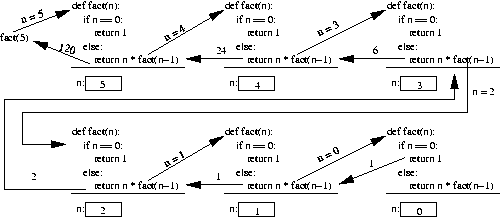
\includegraphics[width=11.5cm]{pic26}
  \end{center}
\end{frame}

\begin{frame}[fragile]
  \frametitle{Primer: obrtanje redosleda znakova u stringu}
  \begin{itemize}
    \item za svaku Python listu na raspolaganju je funkcija \texttt{reverse}
    \item ako hoćemo da konvertujemo string? \\ \ \\
    \item[1] pretvorimo sting u listu znakova
    \item[2] okrenemo listu
    \item[3] pretvorimo listu u string
  \end{itemize}
\end{frame}

\begin{frame}[fragile]
  \frametitle{Primer: obrtanje redosleda znakova u stringu $_2$}
  \begin{itemize}
    \item korišćenjem rekurzije možemo da obavimo ovu operaciju bez pomoćne liste
    \item polazna ideja za rekurziju: \\ \ \\
    \item[1] podelimo string na prvi znak i ostatak stringa
    \item[2] okrenemo ostatak stringa
    \item[3] prvi znak dodamo na kraj okrenutog stringa
  \end{itemize}
\end{frame}

\begin{frame}[fragile]
  \frametitle{Primer: obrtanje redosleda znakova u stringu $_3$}
\begin{minted}{python}
def reverse(s):
    return reverse(s[1:]) + s[0]
\end{minted}
  \begin{itemize}
    \item isečak \texttt{s[1:]} vraća sve osim prvog znaka
    \item okrenemo ovaj isečak i dodamo prvi znak \texttt{s[0]} na kraj 
  \end{itemize}
\end{frame}

\begin{frame}[fragile]
  \frametitle{Primer: obrtanje redosleda znakova u stringu $_4$}
\begin{minted}{python}
>>> reverse("Hello")
...
  File "<stdin>", line 2, in reverse
RuntimeError: maximum recursion depth exceeded
\end{minted}
  \begin{itemize}
    \item šta se desilo?
    \item funkcija ne sadrži osnovni slučaj koji se ne oslanja na rekurziju
    \item funkcija beskonačno poziva samu sebe: svaki poziv \texttt{reverse} dalje poziva \texttt{reverse}
  \end{itemize}
\end{frame}

\begin{frame}[fragile]
  \frametitle{Primer: obrtanje redosleda znakova u stringu $_5$}
  \begin{itemize}
    \item svaki poziv funkcije troši malo memorije
    \item Python zaustavlja rekurziju posle 1000 poziva
    \item šta će biti naš osnovni slučaj?
    \item okretanje praznog stringa daje isti rezultat!
  \end{itemize}
\end{frame}

\begin{frame}[fragile]
  \frametitle{Primer: obrtanje redosleda znakova u stringu $_6$}
\begin{minted}{python}
def reverse(s):
    if s == "":
        return s
    else:
        return reverse(s[1:]) + s[0]

>>> reverse("Hello")
'olleH'
\end{minted}
\end{frame}

\begin{frame}[fragile]
  \frametitle{Primer: anagrami}
  \begin{itemize}
    \item anagram se dobija menjanjem redosleda slova u reči
    \item pravljenje anagrama je specijalni slučaj generisanja svih permutacija nekog niza \\ \ \\
    \item pristup iz prošlog primera:
    \item[1] iseci prvi znak iz stringa
    \item[2] ubaci prvi znak u sve moguće pozicije anagrama koji je dobijen od ostatka stringa
  \end{itemize}
\end{frame}

\begin{frame}[fragile]
  \frametitle{Primer: anagrami $_2$}
  \begin{itemize}
    \item neka je originalni string \texttt{"abc"}
    \item isecanjem \texttt{"a"} ostaje nam \texttt{"bc"}
    \item rezultat generisanja anagrama za \texttt{"bc"} su stringovi \texttt{"bc"} i \texttt{"cb"}
    \item da bismo formirali anagram originalnog stringa, ubacićemo "a" na sve moguće pozicije u okviru dva manja anagrama
    \item \texttt{["abc", "bac", "bca", "acb", "cab", "cba"]}
  \end{itemize}
\end{frame}

\begin{frame}[fragile]
  \frametitle{Primer: anagrami $_2$}
  \begin{itemize}
    \item i u ovom primeru prazan string može poslužiti kao osnovni slučaj za rekurziju
  \end{itemize}
\begin{minted}{python}
def anagrams(s):
    if s == "":
        return [s]
    else:
        ans = []
        for w in anagrams(s[1:]):
            for pos in range(len(w)+1):
                ans.append(w[:pos]+s[0]+w[pos:])
        return ans
\end{minted}
\end{frame}

\begin{frame}[fragile]
  \frametitle{Primer: anagrami $_3$}
  \begin{itemize}
    \item lista se koristi za akumuliranje rezultata
    \item spoljašnja \texttt{for} petlja iterira kroz sve anagrame isečka od \texttt{s}
    \item unutrašnja petlja za svaku poziciju u anagramu ubacuje slovo i kreira novi string
    \item unutrašnja petlja se ponavlja sve do \texttt{len(w)+1} da bi novo slovo moglo da se ubaci i na kraj anagrama
  \end{itemize}
\end{frame}

\begin{frame}[fragile]
  \frametitle{Primer: anagrami $_4$}
\begin{verbatim}
w[:pos]+ s[0] + w[pos:]
\end{verbatim}
  \begin{itemize}
    \item \texttt{w[:pos]} vraća isečak od \texttt{w} sve do (ali ne uključujući) pozicije \texttt{pos}
    \item \texttt{w[pos:]} vraća sve od pozicije \texttt{pos} do kraja
    \item ubacivanje \texttt{s[0]} zapravo ubacuje znak na poziciju \texttt{pos}
    \item unutrašnja petlja se ponavlja sve do \texttt{len(w)+1} da bi novo slovo moglo da se ubaci i na kraj anagrama
  \end{itemize}
\end{frame}

\begin{frame}[fragile]
  \frametitle{Primer: anagrami $_5$}
\begin{minted}{python}
>>> anagrams("abc")
['abc', 'bac', 'bca', 'acb', 'cab', 'cba']
\end{minted}
  \begin{itemize}
    \item broj različitih anagrama jednak je faktorijelu dužine stringa
  \end{itemize}
\end{frame}

\begin{frame}[fragile]
  \frametitle{Primer: brzo stepenovanje}
  \begin{itemize}
    \item jedan način da izračunamo $a^n$ je da pomnožimo $a$ ukupno $n$ puta
    \item ovo se može lako napraviti pomoću akumulatorske petlje:
  \end{itemize}
\begin{minted}{python}
def loopPower(a, n):
    ans = 1
    for i in range(n):
        ans = ans * a
    return ans
\end{minted}
\end{frame}

\begin{frame}[fragile]
  \frametitle{Primer: brzo stepenovanje $_2$}
  \begin{itemize}
    \item ovaj problem možemo rešavati i strategijom podeli-i-vladaj
    \item znamo da je $2^8 = 2^4\cdot 2^4$
    \item ako znamo koliko je $2^4$, možemo izračunati $2^8$ pomoću jednog množenja
    \item dalje, $2^4 = 2^2\cdot 2^2$
    \item dalje $2^2 = 2\cdot 2$ \\ \ \\
    \item izračunali smo $2\cdot 2 = 4$, $4\cdot 4 = 16$, $16\cdot 16 = 256 = 2^8$ pomoću samo tri množenja!
  \end{itemize}
\end{frame}

\begin{frame}[fragile]
  \frametitle{Primer: brzo stepenovanje $_3$}
  \begin{itemize}
    \item znamo da je $a^n = a^{n/2}\cdot a^{n/2}$
    \item šta ako je $n$ neparan broj?
    \item $2^9 = 2^4\cdot 2^4\cdot 2^1$ \\ \ \\
    \item opšti zakon:
  \end{itemize}
    $$ a^n = \left\{
      \begin{array}{ll}
        a^{n//2}\cdot a^{n//2} &\mbox{ ako je $n$ paran broj} \\
        a^{n//2}\cdot a^{n//2}\cdot a &\mbox{ ako je $n$ neparan broj}
      \end{array} 
      \right. $$ \\ \ \\
\end{frame}

\begin{frame}[fragile]
  \frametitle{Primer: brzo stepenovanje $_3$}
  \begin{itemize}
    \item ovde se oslanjamo na celobrojno deljenje: $9//2 = 4$
    \item za rekurzivni algoritam treba nam osnovni slučaj
    \item kako budemo polovili $n$ doći ćemo do nule, jer $1//2=0$
    \item dalje $a^0 = 1$ za svako $a$ osim nule
  \end{itemize}
\end{frame}

\begin{frame}[fragile]
  \frametitle{Primer: brzo stepenovanje $_4$}
\begin{minted}{python}
def recPower(a, n):
    if n ==  0:
        return 1
    else:
        factor = recPower(a, n//2)
        if n%2 == 0:    # n je paran
            return factor * factor
        else:           # n je neparan
            return factor * factor * a
\end{minted}
  \begin{itemize}
    \item \myblue{privremena promenljiva} \texttt{factor} je uvedena da ne bismo dva puta morali da izračunavamo $a^{n//2}$ više od jedanput
  \end{itemize}
\end{frame}

\begin{frame}[fragile]
  \frametitle{Primer: binarna pretraga}
  \begin{itemize}
    \item ispitamo srednji element u listi, i potom pretražujemo donju ili gornju polovinu liste
    \item osnovni slučajevi za rekurziju: kada smo našli podatak ili kada smo suzili pretragu na praznu listu
    \item rekurzivni pozivi će poloviti opseg koji je ,,još u igri``
    \item svaki poziv funkcije će tražiti element između indeksa \texttt{low} i \texttt{high}
  \end{itemize}
\end{frame}

\begin{frame}[fragile]
  \frametitle{Primer: binarna pretraga $_2$}
\begin{minted}{python}
def recBinSearch(x, nums, low, high):
    if low > high:   # nema više gde da se traži
        return -1
    mid = (low + high)//2
    item = nums[mid]
    if item == x:
        return mid
    elif x < item:   # traži u donjoj polovini
        return recBinSearch(x, nums, low, mid-1)
    else:            # traži u gornjoj polovini
        return recBinSearch(x, nums, mid+1, high)
\end{minted}
\end{frame}

\begin{frame}[fragile]
  \frametitle{Primer: binarna pretraga $_3$}
  \begin{itemize}
    \item da bi se prethodna funkcija lakše koristila možemo napraviti novu funkciju koja ,,sakriva`` parametre \texttt{low} i \texttt{high}
  \end{itemize}
\begin{minted}{python}
def search(x, nums):
    return recBinSearch(x, nums, 0, len(nums)-1)
\end{minted}
\end{frame}

\begin{frame}[fragile]
  \frametitle{Rekurzija vs iteracija}
  \begin{itemize}
    \item postoje sličnosti između iteracije (petlje) i rekurzije
    \item sve što se može rešiti pomoću petlje, može i pomoću rekurzije
    \item neki programski jezici imaju samo rekurziju!
    \item neki problemi koji se lako rešavaju rekurzijom su komplikovani za rešavanje petljom
    \item ...i obrnuto
  \end{itemize}
\end{frame}

\begin{frame}[fragile]
  \frametitle{Rekurzija vs iteracija $_2$}
  \begin{itemize}
    \item izračunavanje faktorijela i binarna pretraga na sličan način koriste petlje i rekurziju i efikasnost im je slična
    \item kod stepenovanja je drugačije: 
  \begin{itemize}
    \item verzija sa petljom je linearne složenosti
    \item verzija sa rekurzijom je logaritamske složenosti
    \item razlika u efikasnosti je kao između linearne i binarne pretrage \\ \ \\
  \end{itemize}
    \item da li će rekurzivna rešenja uvek biti brža ili bar jednako brza kao iterativna?
  \end{itemize}
\end{frame}

\begin{frame}[fragile]
  \frametitle{Rekurzija vs iteracija $_3$}
  \begin{itemize}
    \item Fibonačijevi brojevi predstavljaju niz 1,1,2,3,5,8,...
  \begin{itemize}
    \item sekvenca počinje sa 1,1
    \item sledeći broj se računa kao zbir prethodna dva
  \end{itemize}
  \end{itemize}
\end{frame}

\begin{frame}[fragile]
  \frametitle{Fibonacci iterativno}
  \begin{itemize}
    \item promenljive \texttt{curr} i \texttt{prev} služe za računanje sledećeg broja u nizu
    \item kada ga izračunamo, postavimo \texttt{prev} na \texttt{curr} i \texttt{curr} na novoizračunati broj
    \item stavimo ovo u petlju i izvršimo potreban broj ciklusa
  \end{itemize}
\end{frame}

\begin{frame}[fragile]
  \frametitle{Fibonacci iterativno $_2$}
\begin{minted}{python}
def loopfib(n):
    curr = 1
    prev = 1
    for i in range(n-2):
        curr, prev = curr+prev, curr
    return curr
\end{minted}
  \begin{itemize}
    \item iskoristili smo dvostruku dodelu
    \item petlja izvršava $n-2$ ciklusa jer prva dva broja već imamo
  \end{itemize}
\end{frame}

\begin{frame}[fragile]
  \frametitle{Fibonacci rekurzivno}
$$ fib(n) = \left\{
  \begin{array}{ll}
    1 &\mbox{ako je $n<3$} \\
    fib(n-1)+fib(n-2) &\mbox{ina\v{c}e}
  \end{array} 
  \right. $$
  \begin{itemize}
    \item lako je napisati funkciju na osnovu ovakve definicije:
  \end{itemize}
\begin{minted}{python}
def fib(n):
    if n < 3:
        return 1
    else:
        return fib(n-1)+fib(n-2)
\end{minted}
\end{frame}

\begin{frame}[fragile]
  \frametitle{Fibonacci rekurzivno $_2$}
  \begin{itemize}
    \item ova funkcija poštuje sva pravila koja smo ranije postavili:
  \begin{itemize}
    \item rekurzija se zasniva na manjim vrednostima
    \item postoji osnovni slučaj koji se ne oslanja na rekurziju
  \end{itemize}
    \item da li će rekurzivna varijanta raditi efikasno?...
  \end{itemize}
\end{frame}

\begin{frame}[fragile]
  \frametitle{Fibonacci rekurzivno $_3$}
  \begin{itemize}
    \item rekurzivno rešenje je neefikasno jer obavlja puno ponovljenih izračunavanja!
  \end{itemize}
\begin{center}
  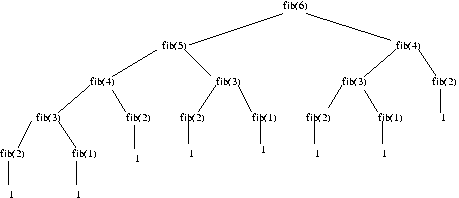
\includegraphics[width=10cm]{pic27}
\end{center}
\end{frame}

\begin{frame}[fragile]
  \frametitle{Fibonacci rekurzivno $_4$}
  \begin{itemize}
    \item da bismo izračunali \texttt{fib(6)}, \texttt{fib(4)} će se računati dva puta, 
      \texttt{fib(3)} će se računati 3 puta, \texttt{fib(2)} će se računati 4 puta...
    \item za velike brojeve ima jako puno ponovljenih proračuna
  \end{itemize}
\begin{center}
  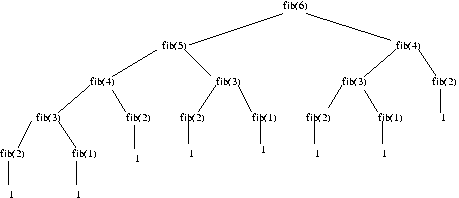
\includegraphics[width=10cm]{pic27}
\end{center}
\end{frame}

\begin{frame}[fragile]
  \frametitle{Rekurzija vs iteracija}
  \begin{itemize}
    \item rekurzija je još jedan alat za rešavanje problema
    \item ponekad je rekurzija efikasnija od iterativnog rešenja
    \item u drugim slučajevima, kada su rešenja slična, iterativno rešenje je obično brže
    \item rekurzivna rešenja treba izbegavati ako su neefikasna, ili kada ne možemo napraviti iterativno rešenje
  \end{itemize}
\end{frame}

\section{Sortiranje}

\begin{frame}[fragile]
  \frametitle{Algoritmi za sortiranje}
  \begin{itemize}
    \item osnovni problem sortiranja: 
    \item prerasporediti elemente liste tako da su poređani u rastućem ili opadajućem redosledu
  \end{itemize}
\end{frame}

\begin{frame}[fragile]
  \frametitle{Selection sort}
  \begin{itemize}
    \item dat nam je špil karata koje treba da poređamo u rastućem redosledu
    \item kako da to uradimo?
    \item pronađemo najmanju kartu (sekvencijalno) i stavimo je na vrh špila
    \item ponovimo postupak za ostatak špila
    \item sve ovo ponavljamo dok ne sortiramo ceo špil \\ \ \\
    \item ovaj algoritam je poznat kao \myblue{selection sort}
  \end{itemize}
\end{frame}

\begin{frame}[fragile]
  \frametitle{Selection sort $_2$}
  \begin{itemize}
    \item algoritam ima petlju
    \item u svakom ciklusu nađemo najmanji element i premestimo ga na početak
  \begin{itemize}
    \item za svih $n$ elemenata: nađemo najmanji i premestimo ga na \myblue{nultu} poziciju
    \item za elemente sa pozicijama $1$ do $n-1$: nađemo najmanji i premestimo ga na \myblue{prvu} poziciju
    \item za elemente sa pozicijama $2$ do $n-1$: nađemo najmanji i premestimo ga na \myblue{drugu} poziciju
    \item ...
  \end{itemize}
  \end{itemize}
\end{frame}

\begin{frame}[fragile]
  \frametitle{Selection sort $_3$}
  \begin{itemize}
    \item kada premeštamo element na nultu poziciju, ne smemo da izgubimo element koji se tamo nalazi!
    \item možemo da im zamenimo mesta: \\
      \texttt{nums[0], nums[x] = nums[x], nums[0]}
    \item možemo da implementiramo algoritam:
    \item \texttt{bottom} je pozicija za najmanji element
    \item \texttt{mp} je pozicija najmanjeg koga smo pronašli
  \end{itemize}
\end{frame}

\begin{frame}[fragile]
  \frametitle{Selection sort $_4$}
\begin{minted}{python}
def selectionSort(nums):
    n = len(nums)
    for bottom in range(n-1):
        mp = bottom         # bottom je trenutno najmanji
        for i in range(bottom+1, n): # za svaku poziciju
            if nums[i] < nums[mp]:   # ako je manji
                mp = i               # zapamti mu indeks

        # zameni mesta
        nums[bottom], nums[mp] = nums[mp], nums[bottom]
\end{minted}
\end{frame}

\begin{frame}[fragile]
  \frametitle{Selection sort $_4$}
  \begin{itemize}
    \item umesto da pamtimo najmanju vrednost, pamtimo joj \myblue{poziciju} u promenljivoj \texttt{mp}
    \item nove vrednosti se testiraju poređenjem elementa sa indeksom \texttt{i} i elementa sa indeksom \texttt{mp}
    \item \texttt{bottom} se zaustavlja na indeksu \texttt{n-2}: kada nam ostane samo jedan element, on je i najveći!
  \end{itemize}
\end{frame}

\begin{frame}[fragile]
  \frametitle{Selection sort $_5$}
  \begin{itemize}
    \item selection sort se lako implementira
    \item pristojno radi za liste skromne dužine
    \item nije efikasan
  \end{itemize}
\end{frame}

\begin{frame}[fragile]
  \frametitle{Merge sort}
  \begin{itemize}
    \item primena podeli-i-vladaj pristupa na sortiranje
    \item recimo da smo dobili špil karata da sortiramo
    \item[1] podelimo špil na dva dela
    \item[2] sortiramo prvu polovinu
    \item[3] sortiramo drugu polovinu
    \item[4] spojimo dve sortirane polovine (tako da rezultat bude sortiran)
  \end{itemize}
\end{frame}

\begin{frame}[fragile]
  \frametitle{Merge sort $_2$}
  \begin{itemize}
    \item proces kombinovanja dve sortirane liste u jednu zove se spajanje (\myblue{merging})
    \item korak 1: podeli špil na dva dela
  \begin{itemize}
    \item ovo je lako: koristićemo isecanje liste
  \end{itemize}
    \item korak 4: spajanje sortiranih polovina
  \begin{itemize}
    \item uporedimo dve karte na vrhu svake polovine; manja od njih će biti na vrhu celog špila
    \item kada sklonimo najmanju kartu, ponovo poredimo najmanje karte u obe polovine
    \item ponavljamo postupak dok ne potrošimo jednu polovinu; ostatak druge polovine dodamo na kraj špila
  \end{itemize}
  \end{itemize}
\end{frame}

\begin{frame}[fragile]
  \frametitle{Merge sort $_3$}
  \begin{itemize}
    \item \texttt{lst1} i \texttt{lst2} su dve pod-liste
    \item \texttt{lst3} je rezultat
  \end{itemize}
\end{frame}

\begin{frame}[fragile]
  \frametitle{Merge sort $_4$}
\begin{minted}{python}
def merge(lst1, lst2, lst3):
    # indeksi tekućih pozicija u svakoj od lista
    i1, i2, i3 = 0, 0, 0  # svi počinju od početka
    n1, n2 = len(lst1), len(lst2)

    # dok u obe polovine ima elemenata
    while i1 < n1 and i2 < n2:
        if lst1[i1] < lst2[i2]: # vrh iz lst1 je manji
            lst3[i3] = lst1[i1] # kopiraj ga u lst3 na kraj
            i1 = i1 + 1
        else:                   # vrh iz lst2 je manji
            lst3[i3] = lst2[i2] # kopiraj ga u lst3 na kraj
            i2 = i2 + 1
        i3 = i3 + 1             # pomeri indeks za lst3
\end{minted}
\end{frame}

\begin{frame}[fragile]
  \frametitle{Merge sort $_5$}
\begin{minted}{python}
# Sada smo ispraznili lst1 ili lst2. Iskopiraj ostatak iz
# liste koja nije prazna u lst3.

    # kopiraj elemente iz lst1 ako ih ima
    while i1 < n1:
        lst3[i3] = lst1[i1]
        i1 = i1 + 1
        i3 = i3 + 1

    # kopiraj elemente iz lst2 ako ih ima
    while i2 < n2:
        lst3[i3] = lst2[i2]
        i2 = i2 + 1
        i3 = i3 + 1
\end{minted}
\end{frame}

\begin{frame}[fragile]
  \frametitle{Merge sort $_6$}
  \begin{itemize}
    \item možemo da podelimo listu na polovine
    \item i da spojimo podeljene liste nazad
    \item kako da sortiramo polovine? -- novim deljenjem
    \item liči na rekurziju! \\ \ \\
    \item treba nam osnovni slučaj kada rekurzija prestaje
    \item i da rekurzivni pozivi uvek operišu nad manjom varijantom početnog problema
  \end{itemize}
\end{frame}

\begin{frame}[fragile]
  \frametitle{Merge sort $_7$}
  \begin{itemize}
    \item na kraju deobe ćemo doći do liste dužine 1
    \item ta lista je sortirana!
    \item da skiciramo rekurziju:
  \end{itemize}
\begin{minted}{python}
if len(nums) > 1:
    podeli listu na dva dela
    mergeSort(prva polovina)
    mergeSort(druga polovina)
    spoj dve liste u jednu
\end{minted}
\end{frame}

\begin{frame}[fragile]
  \frametitle{Merge sort $_8$}
\begin{minted}{python}
def mergeSort(nums):
    n = len(nums)
    if n > 1:
        m = n//2
        nums1, nums2 = nums[:m], nums[m:]
        mergeSort(nums1)
        mergeSort(nums2)
        merge(nums1, nums2, nums)
\end{minted}
\end{frame}

\begin{frame}[fragile]
  \frametitle{Selection sort vs merge sort}
  \begin{itemize}
    \item imamo dva algoritma za sortiranje; koji da koristimo?
    \item složenost postupka sortiranja zavisi od dužine liste
    \item treba da odredimo u koliko koraka svaki algoritam obavi sortiranje
  \end{itemize}
\end{frame}

\begin{frame}[fragile]
  \frametitle{Selection sort vs merge sort $_2$}
  \begin{itemize}
    \item da krenemo sa selection sortom
    \item lista je dužine $n$
    \item za pronalaženje najmanjeg elementa, testiramo svih $n$ elemenata
    \item u sledećem ciklusu testiramo $n-1$ elemenata
    \item u sledećem ciklusu testiramo $n-2$ elemenata
    \item ...
    \item ukupan broj iteracija je: \\
      $$ n + (n-1) + (n-2) + (n-3) + \ldots + 1 $$
  \end{itemize}
\end{frame}

\begin{frame}[fragile]
  \frametitle{Selection sort vs merge sort $_3$}
  \begin{itemize}
    \item vreme potrebno selection sortu da sortira listu dužine $n$
    \item je proporcionalno sumi prvih $n$ prirodnih brojeva, odnosno \\
      $$ \frac{n(n+1)}{2} $$
    \item u ovoj formuli se pojavljuje $n^2$
    \item što znači da je broj potrebnih koraka \myblue{proporcionalan kvadratu} dužine liste
    \item $\rightarrow$ algoritam kvadratne složenosti
  \end{itemize}
\end{frame}

\begin{frame}[fragile]
  \frametitle{Selection sort vs merge sort $_4$}
  \begin{itemize}
    \item sada analiziramo merge sort
    \item lista se podeli na dve polovine, svaka se sortira i potom se spoje
    \item pravo mesto gde se sortiranje odvija je funkcija \texttt{merge}
    \item ova slika pokazuje kako se sortira lista \texttt{[3,1,4,1,5,9,2,6]}
    \item idući od dole, treba da kopiramo $n$ vrednosti u drugi nivo
  \end{itemize}
\begin{center}
  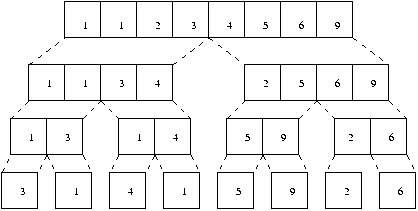
\includegraphics[width=6cm]{pic28}
\end{center}
\end{frame}

\begin{frame}[fragile]
  \frametitle{Selection sort vs merge sort $_5$}
  \begin{itemize}
    \item od drugog prema trećem nivou treba opet kopirati $n$ vrednosti
    \item svaki nivo podrazumeva kopiranje $n$ vrednosti
    \item koliko ima nivoa?
    \item na osnovu analize binarne pretrage, znamo da ih ima $log_2 n$
    \item ukupan broj koraka za sortiranje je $n\cdot log_2 n$
  \end{itemize}
\begin{center}
  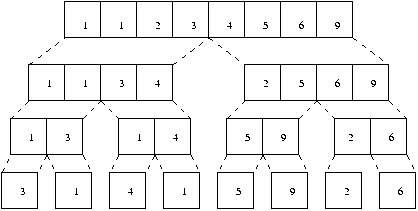
\includegraphics[width=6cm]{pic28}
\end{center}
\end{frame}

\begin{frame}[fragile]
  \frametitle{Selection sort vs merge sort $_6$}
  \begin{itemize}
    \item koji algoritam je bolji: selection sa $n^2$ ili merge sa $n log_2 n$ operacija?
    \item za kratke liste selection sort može biti brži jer je kôd jednostavniji
    \item kada $n$ poraste...
    \item funkcija $n log_2 n$ raste znatno sporije od $n^2$
  \end{itemize}
\end{frame}

\begin{frame}[fragile]
  \frametitle{Selection sort vs merge sort $_7$}
\begin{center}
  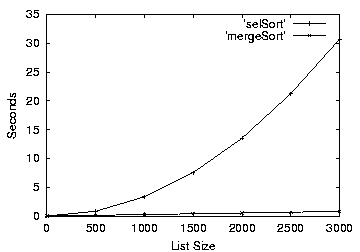
\includegraphics[width=9cm]{pic29}
\end{center}
\end{frame}

\section{Složeni problemi}

\begin{frame}[fragile]
  \frametitle{Složeni problemi}
  \begin{itemize}
    \item pomoću podeli-i-vladaj pristupa možemo napraviti efikasne algoritme za sortiranje i pretragu
    \item podeli-i-vladaj i rekurzija su moćne tehnike za dizajn algoritama
    \item ali nemaju svi problemi efikasno rešenje!
  \end{itemize}
\end{frame}

\begin{frame}[fragile]
  \frametitle{Hanojske kule}
  \begin{itemize}
    \item imamo tri stuba i 64 koncentrična diska različitih prečnika, poređanih u obliku kupe
    \item treba premestiti diskove sa jednog stuba na drugi pomoću tri pravila:
  \begin{itemize}
    \item samo jedan disk može da se pomera u jednom trenutku
    \item disk se sme spustiti samo na stub, ne može se ostaviti sa strane
    \item veći disk se ne sme spustiti na manji
  \end{itemize}
  \end{itemize}
\begin{center}
  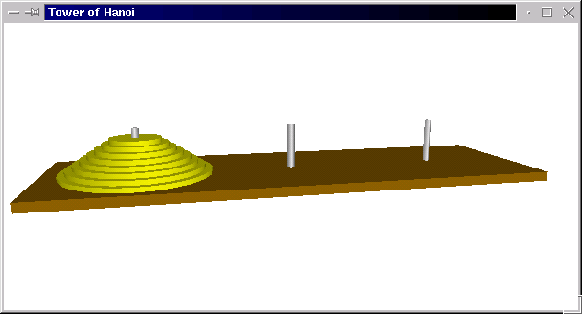
\includegraphics[width=7cm]{pic30}
\end{center}
\end{frame}

\begin{frame}[fragile]
  \frametitle{Hanojske kule $_2$}
  \begin{itemize}
    \item ako stubove označimo sa A, B i C
    \item operacije za premeštanje su
  \begin{itemize}
    \item premesti disk sa A na C
    \item premesti disk sa A na B
    \item premesti disk sa C na B
  \end{itemize}
  \end{itemize}
\begin{center}
  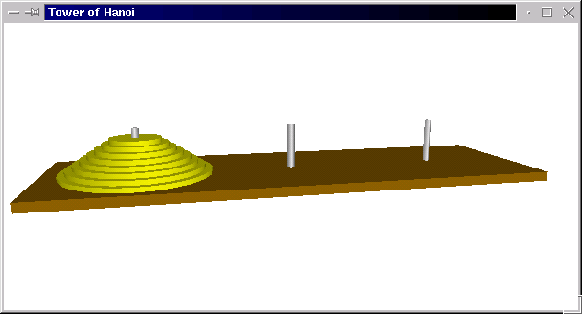
\includegraphics[width=7cm]{pic30}
\end{center}
\end{frame}

\begin{frame}[fragile]
  \frametitle{Hanojske kule $_3$}
  \begin{itemize}
    \item jednostavni slučajevi:
    \item 1 disk
  \begin{itemize}
    \item premesti disk sa A na C
  \end{itemize}
    \item 2 diska
  \begin{itemize}
    \item premesti disk sa A na B
    \item premesti disk sa A na C
    \item premesti disk sa B na C
  \end{itemize}
  \end{itemize}
\end{frame}

\begin{frame}[fragile]
  \frametitle{Hanojske kule $_4$}
  \begin{itemize}
    \item 3 diska
  \begin{itemize}
    \item da bismo premestili najveći na C, treba prvo da sklonimo 2 manja diska
    \item ova dva diska čine kupu visine 2, što znamo da rešimo
  \end{itemize}
  \end{itemize}
\end{frame}

\begin{frame}[fragile]
  \frametitle{Hanojske kule $_5$}
  \begin{itemize}
    \item algoritam: premesti kulu sa $n$ diskova
  \begin{itemize}
    \item[1] premesti kulu visine $n-1$ sa početnog položaja na pomoćni
    \item[2] premesti kulu visine $1$ na krajnji položaj
    \item[3] premesti kulu visine $n-1$ sa pomoćnog položaja na krajnji
  \end{itemize}
    \item osnovni slučaj: premeštanje kule visine $1$
  \end{itemize}
\end{frame}

\begin{frame}[fragile]
  \frametitle{Hanojske kule $_6$}
  \begin{itemize}
    \item \texttt{n} je visina kule
    \item \texttt{source}, \texttt{dest}, \texttt{temp} su tri stuba
  \end{itemize}
\begin{minted}{python}
def moveTower(n, source, dest, temp):
    if n == 1:
        print("Premesti disk sa", source, "na", dest+".")
    else:
        moveTower(n-1, source, temp, dest)
        moveTower(1, source, dest, temp)
        moveTower(n-1, temp, dest, source)
\end{minted}
\end{frame}

\begin{frame}[fragile]
  \frametitle{Hanojske kule $_7$}
  \begin{itemize}
    \item napravimo funkciju koja započinje postupak
  \end{itemize}
\begin{minted}{python}
def hanoi(n):
    moveTower(n, "A", "C", "B")

>>> hanoi(3)
Premesti disk sa A na C.
Premesti disk sa A na B.
Premesti disk sa C na B.
Premesti disk sa A na C.
Premesti disk sa B na A.
Premesti disk sa B na C.
Premesti disk sa A na C.
\end{minted}
\end{frame}

\begin{frame}[fragile]
  \frametitle{Hanojske kule $_8$}
  \begin{itemize}
    \item ovo je ,,složen problem``
    \item za visinu kule $n$ treba nam $2^n-1$ koraka
  \end{itemize}
\begin{center}
\begin{tabular}{cc}
\textbf{diskova} & \textbf{koraka} \\ \hline
1 & 1 \\
2 & 3 \\
3 & 7 \\
4 & 15 \\
5 & 31
\end{tabular}
\end{center}
\end{frame}

\begin{frame}[fragile]
  \frametitle{Hanojske kule $_8$}
  \begin{itemize}
    \item algoritam ima \myblue{eksponencijalnu} složenost
    \item potrebno vreme raste veoma brzo sa $n$ \\ \ \\
    \item za 64 diska, pomerajući jedan u sekundi, potrebno je 580 milijardi godina da se završi
    \item (starost svemira je oko 15 milijardi godina)
  \end{itemize}
\end{frame}

\begin{frame}[fragile]
  \frametitle{Hanojske kule $_9$}
  \begin{itemize}
    \item algoritam za hanojske kule se lako definiše
    \item ali je neupotrebljiv za rešavanje problema osim za trivijalne slučajeve -- \myblue{intractable}
    \item postoje problemi koji su još složeniji
  \end{itemize}
\end{frame}

\begin{frame}[fragile]
  \frametitle{Problem zaustavljanja}
  \begin{itemize}
    \item pišemo program koji analizira druge programe i određuje da li imaju beskonačnu petlju
    \item znamo i ulaz u program koji analiziramo
    \item da izbegnemo slučaj da program ima beskonačnu petlju zbog određene kombinacije ulaznih podataka
  \end{itemize}
\end{frame}

\begin{frame}[fragile]
  \frametitle{Problem zaustavljanja $_2$}
  \begin{itemize}
    \item specifikacija programa
  \begin{itemize}
    \item ulaz: fajl sa Python programom; ulazni podaci za njega
    \item izlaz: \texttt{"OK"} ako će se program zaustaviti, \texttt{"FAULT"} ako ima beskonačnu petlju 
  \end{itemize}
  	\item npr. Python interpreter je program koji analizira programe!
  	\item program i njegovi ulazi se mogu predstaviti kao stringovi
  \end{itemize}
\end{frame}

\begin{frame}[fragile]
  \frametitle{Problem zaustavljanja $_3$}
  \begin{itemize}
    \item \myblue{ne postoji algoritam} koji može ispuniti ovu specifikaciju!
    \item nije isto kao kada kažemo da niko ne može da ga napiše
    \item možemo dokazati ovu tvrdnju matematičkom tehnikom koja se zove \myblue{dokaz kontradikcijom}
  \end{itemize}
\end{frame}

\begin{frame}[fragile]
  \frametitle{Problem zaustavljanja $_4$}
  \begin{itemize}
    \item dokaz kontradikcijom: pretpostavićemo da važi suprotno od onoga što želimo da dokažemo
    \item ako nas ta pretpostavka dovede u kontradikciju, to znači da pretpostavka nije tačna
    \item tada će biti tačno ono što smo želeli da dokažemo
  \end{itemize}
\end{frame}

\begin{frame}[fragile]
  \frametitle{Problem zaustavljanja $_5$}
  \begin{itemize}
    \item pretpostavimo da postoji algoritam koji može da odredi da li se neki program završava za date ulazne podatke
    \item ako postoji, možemo ga zapisati kao funkciju:
  \end{itemize}
\begin{minted}{python}
# turing.py

def terminates(program, inputData):
    # program i inputData su stringovi
    # vraća True ako će se program zaustaviti kada mu se
    # daju inputData kao ulazni podaci
\end{minted}
\end{frame}

\begin{frame}[fragile]
  \frametitle{Problem zaustavljanja $_6$}
\begin{minted}{python}
def main():
    lines = []
    print("Ukucaj program ('done' za kraj).")
    line = input("")
    while line != "done":
        lines.append(line)
        line = input("")
    testProg = "\n".join(lines)

    # ako se program zaustavi kad dobije samog sebe 
    # kao ulazne podatke, uđi u beskonačnu petlju
    if terminates(testProg, testProg):
        while True:
            pass        # pass naredba ne radi ništa
\end{minted}
\end{frame}

\begin{frame}[fragile]
  \frametitle{Problem zaustavljanja $_7$}
  \begin{itemize}
    \item prvo unosimo program sa tastature, pomoću sentinel petlje
    \item \texttt{join} funkcija spaja sve redove stavljajući \texttt{$\backslash$n} između njih
    \item dobili smo višelinijski string koji sadrži ukucani program
  \end{itemize}
\end{frame}

\begin{frame}[fragile]
  \frametitle{Problem zaustavljanja $_8$}
  \begin{itemize}
    \item \texttt{turing.py} koristi ovaj program za testiranje, ali koristi ga i kao ulazne podatke
    \item dakle, proveravamo da li će se program zaustaviti ako mu prosledimo samoga sebe kao ulaz
    \item ako se program zaustavi, \texttt{turing.py} će ući u beskonačnu petlju
  \end{itemize}
\end{frame}

\begin{frame}[fragile]
  \frametitle{Problem zaustavljanja $_9$}
  \begin{itemize}
    \item ovo je sve uvod u glavno pitanje:
    \item šta će se desiti kada pokrenemo \texttt{turing.py} i damo mu \texttt{turing.py} da ga analizira?
    \item da li se \texttt{turing.py} zaustavlja kada dobije samog sebe kao ulaz?
  \end{itemize}
\end{frame}

\begin{frame}[fragile]
  \frametitle{Problem zaustavljanja $_{10}$}
  \begin{itemize}
    \item u funkciji \texttt{terminates} se određuje da li će se program zaustaviti
    \item dva moguća slučaja:
  \begin{itemize}
    \item[1] \texttt{turing.py} će se \textbf{zaustaviti} kada mu damo njega samog kao ulaz
  \begin{itemize}
    \item funkcija \texttt{terminates} vraća \texttt{True}
    \item \texttt{turing.py} potom ulazi u beskonačnu petlju
    \item prema tome, \texttt{turing.py} se \textbf{ne zaustavlja} -- kontradikcija
  \end{itemize}
    \item[2] \texttt{turing.py} će se \textbf{neće zaustaviti} kada mu damo njega samog kao ulaz
  \begin{itemize}
    \item funkcija \texttt{terminates} vraća \texttt{False}
    \item kada \texttt{terminates} vrati \texttt{False}, \texttt{turing.py} se završava
    \item \texttt{turing.py} se \textbf{zaustavio} -- kontradikcija
  \end{itemize}
  \end{itemize}
  \end{itemize}
\end{frame}

\begin{frame}[fragile]
  \frametitle{Problem zaustavljanja $_{11}$}
  \begin{itemize}
    \item pretpostavka da postoji funkcija \texttt{terminates} nas je dovela u kontradikciju
    \item $\Rightarrow$ takva funkcija ne postoji!
  \end{itemize}
\end{frame}

\begin{frame}[fragile]
  \frametitle{Glava}
  \begin{itemize}
    \item najvažniji kompjuter koji programer ima je onaj između ušiju
  \end{itemize}
\end{frame}

\end{document}